% SPDX-License-Identifier: CC-BY-SA-4.0
% Author: Matthieu Perrin
% Part: 
% Section: 
% Sub-section: 
% Frame: 

\begingroup

\begin{frame}{Arbre de la syntaxe abstraite}
  \small
  \vspace{-2mm}  \begin{block}{Arbre de la syntaxe abstraite (AST)}
    \begin{itemize}
    \item\vspace{-2mm} Les arbres de dérivation peuvent être simplifiés en un AST
      \begin{description}
      \item[N\oe uds :] Constructions du langage (souvent des opérateurs)
      \item[Feuilles :] Constantes ou variables
      \end{description}
    \item\vspace{-1mm} La suite de la compilation utilise un AST. Par exemple, en Bison

      \texttt{S:    `(' S `+' S `)'    \{\$\$ = new Sum(\$2, \$4);\}}
    \end{itemize}
  \end{block}

  \vspace{-2mm}\begin{exampleblock}{Exemple}
    Génération du mot $u=\example{((1+1)\times (1+1))}$ par la grammaire $G = \langle \{\example{1}, \example{+}, \example{\times}, \example{(}, \example{)}\}, \{S\}, S, \{S \rightarrow \example{(}S \example{+} S\example{)} | \example{(}S \example{\times} S\example{)} | \example{1} \} \rangle$.

    \begin{minipage}[t]{.5\textwidth}
      \example{Arbre de la syntaxe concrète}\\
      \scalebox{.75}{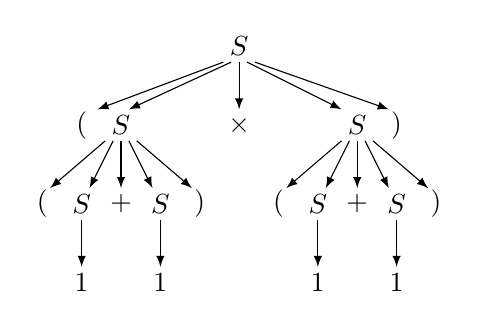
\begin{tikzpicture}
          \draw (3.5,3.0) node{$S$};
          \draw (1.5,2.0) node{$($};
          \draw (2.0,2.0) node{$S$};
          \draw (3.5,2.0) node{$\times$};
          \draw (5.0,2.0) node{$S$};
          \draw (5.5,2.0) node{$)$};
          \draw (1.0,1.0) node{$($};
          \draw (1.5,1.0) node{$S$};
          \draw (2.0,1.0) node{$+$};
          \draw (2.5,1.0) node{$S$};
          \draw (3.0,1.0) node{$)$};
          \draw (4.0,1.0) node{$($};
          \draw (4.5,1.0) node{$S$};
          \draw (5.0,1.0) node{$+$};
          \draw (5.5,1.0) node{$S$};
          \draw (6.0,1.0) node{$)$};
          \draw (1.5,0.0) node{$1$};
          \draw (2.5,0.0) node{$1$};
          \draw (4.5,0.0) node{$1$};
          \draw (5.5,0.0) node{$1$};

          \draw[-latex] (3.3,2.8) -- (1.7,2.2) ; 
          \draw[-latex] (3.4,2.8) -- (2.1,2.2) ; 
          \draw[-latex] (3.5,2.8) -- (3.5,2.2) ; 
          \draw[-latex] (3.6,2.8) -- (4.8,2.2) ; 
          \draw[-latex] (3.7,2.8) -- (5.4,2.2) ; 
          \draw[-latex] (1.8,1.8) -- (1.1,1.2) ; 
          \draw[-latex] (1.9,1.8) -- (1.6,1.2) ; 
          \draw[-latex] (2.0,1.8) -- (2.0,1.2) ; 
          \draw[-latex] (2.1,1.8) -- (2.4,1.2) ; 
          \draw[-latex] (2.2,1.8) -- (2.9,1.2) ; 
          \draw[-latex] (4.8,1.8) -- (4.1,1.2) ; 
          \draw[-latex] (4.9,1.8) -- (4.6,1.2) ; 
          \draw[-latex] (5.0,1.8) -- (5.0,1.2) ; 
          \draw[-latex] (5.1,1.8) -- (5.4,1.2) ; 
          \draw[-latex] (5.2,1.8) -- (5.9,1.2) ; 
          \draw[-latex] (1.5,0.8) -- (1.5,0.2) ; 
          \draw[-latex] (2.5,0.8) -- (2.5,0.2) ; 
          \draw[-latex] (4.5,0.8) -- (4.5,0.2) ; 
          \draw[-latex] (5.5,0.8) -- (5.5,0.2) ; 
      \end{tikzpicture}}
    \end{minipage}%
    \begin{minipage}[t]{.5\textwidth}
      \example{Arbre de la syntaxe abstraite}\\
      \scalebox{.75}{\begin{tikzpicture}
          \draw (3.0,2.0) node{$\times$};
          \draw (1.0,1.0) node{$+$};
          \draw (5.0,1.0) node{$+$};
          \draw (0.0,0.0) node{$1$};
          \draw (2.0,0.0) node{$1$};
          \draw (4.0,0.0) node{$1$};
          \draw (6.0,0.0) node{$1$};

          \draw[-latex] (2.6,1.8) -- (1.4,1.2); 
          \draw[-latex] (3.4,1.8) -- (4.6,1.2); 
          \draw[-latex] (0.8,0.8) -- (0.2,0.2); 
          \draw[-latex] (1.2,0.8) -- (1.8,0.2); 
          \draw[-latex] (4.8,0.8) -- (4.2,0.2); 
          \draw[-latex] (5.2,0.8) -- (5.8,0.2); 
      \end{tikzpicture}}
    \end{minipage}
  \end{exampleblock}
\end{frame}

\endgroup
